%!TEX root = ../project.tex
\part{Design}

Now that we have analysed the problem, we can begin to design the program,
including this like; the flow of data, what the interface will look like and how
the program will function.

%%%
\section{Overall System Design}

\begin{tabular}{llll}
	Inputs & Processes & Storage & Outputs \\ \hline
	Body Parameters & Trajectory Calculations 
		& Current State & Graphical Output \\
	Number of Bodies & Position Calculations 
		& Initial State & Coordinates of Bodies \\ 
	& Graphical Processing && Velocity of Bodies \\
\end{tabular}

%%%
\section{Human Computer Interface}

\begin{figure}[h!]
	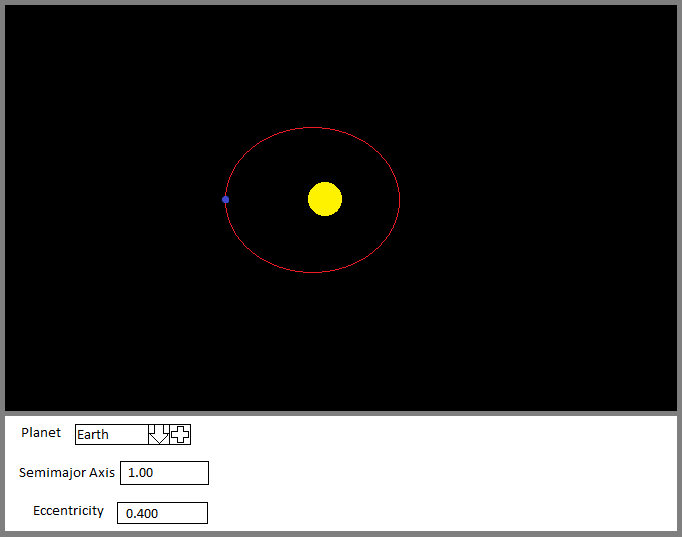
\includegraphics[width=\textwidth]{./img/interface.png}
	\caption{A mockup of the interface}
	\label{fig:hci}
\end{figure}

This is a basic mock-up of what I intend for the interface to look like. It looks
quite similar to the old system's interface, so it will be familiar to the user
and they won't have to learn a lot in order to use it.

%%%
\section{Hardware Specification}

My program needs to run on the computers at school, which have:
\begin{description}
	\item[Processor:] Intel Core i3 @ 3.3GHz
	\item[RAM:] 4GB
	\item[Graphics:] Intel HD 2000
	\item[Operating System:] Windows 7
\end{description}

The program will also need basic input and output devices, a monitor, keyboard
and mouse. A projector is also recommended for using the program to explain
Kepler's laws in front of a class.

%%%
\section{System Flowchart}

\begin{figure}[H]
	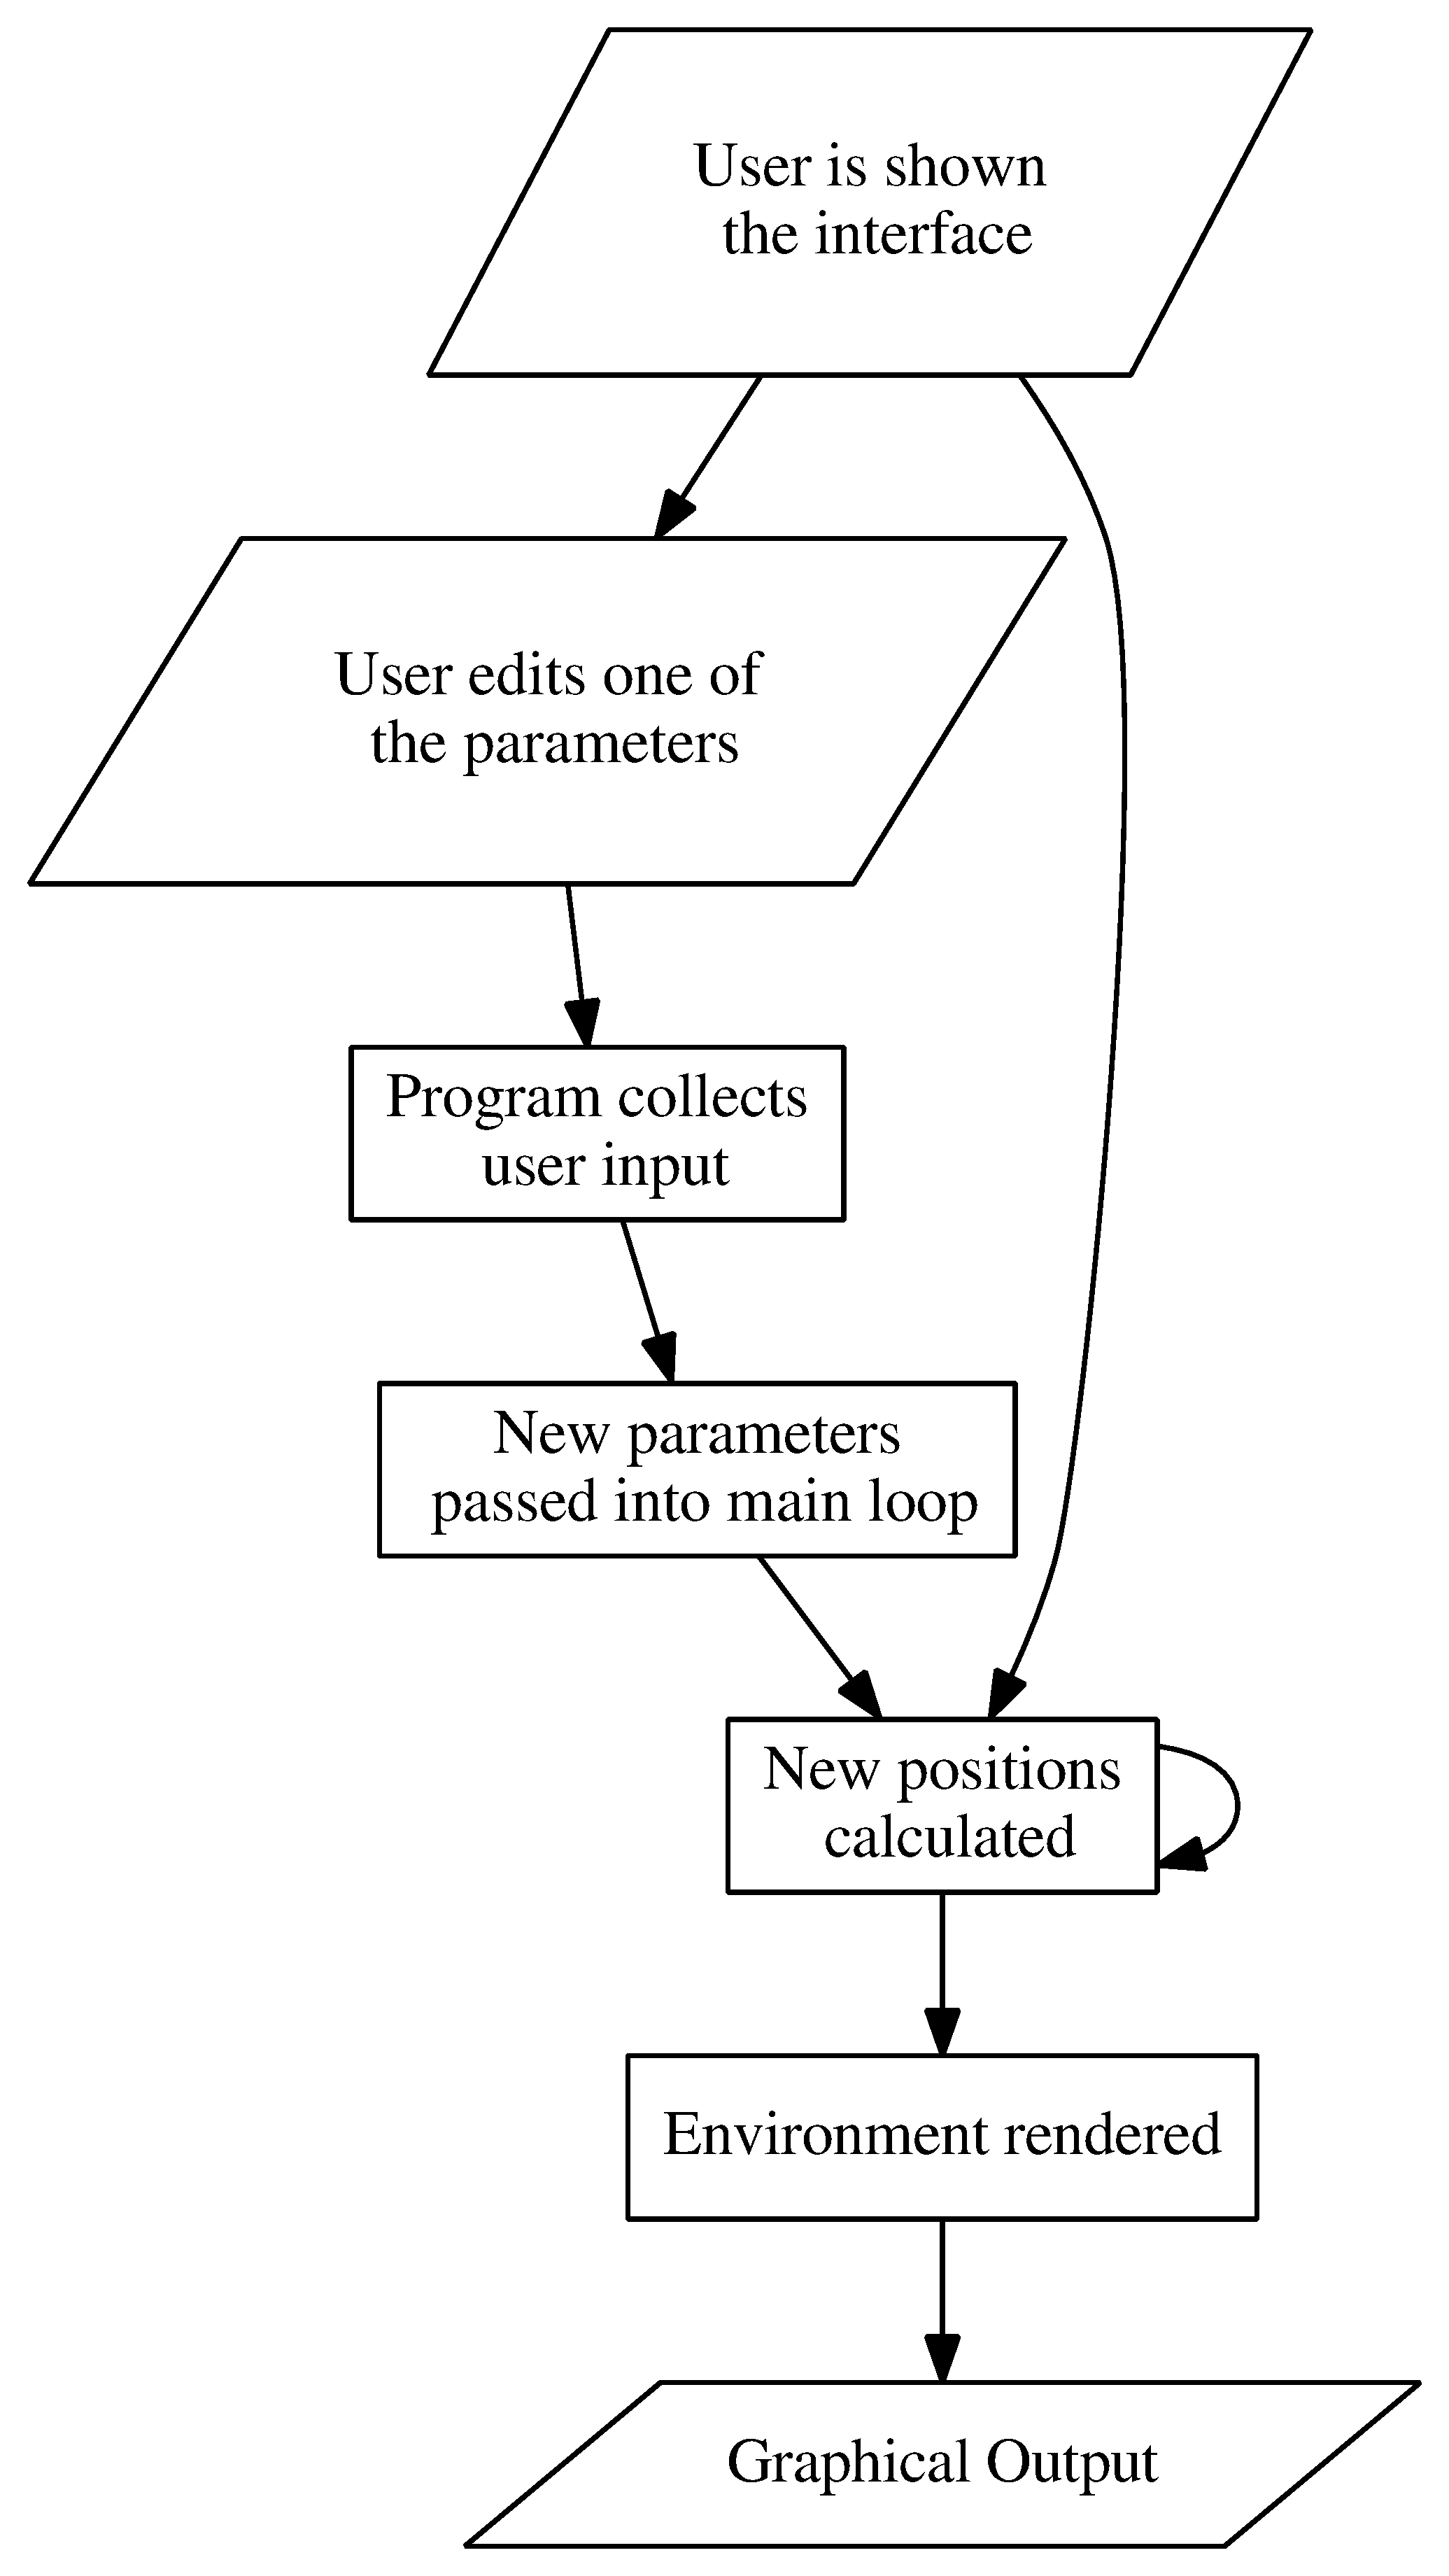
\includegraphics[scale=0.2]{./img/flow.eps}
	\label{fig:flow}	
\end{figure}

%%%
\section{Possible Algorithms to Use}

A big part of my program is the actual simulation of the orbits of some
simulated planets. To simulate and orbit a complex algorithm is required, and
there's a few different ones to choose from. \\

The Barnes-Hut Tree is a method for performing N-Body simulations, which means
that every body in the simulation will be interacting with every other body.
This, however, isn't very useful for a basic model of a simulation of a solar
system, as the planets generally don't interact with each other very much. It
will allow for more complex simulations, but this isn't necessary for my
project. \\

The simulation can be simplified to a two body problem, between one planet and
the sun, because the planets aren't affecting each other. This can then be
further simplified to a one body problem, because the sun is much more massive
than a planet, so it can be thought of as the centre of mass. \\

Newton's \emph{law of universal gravitation} states that two bodies, with masses
$m_1$ and $m_2$, separated my $r$ are attracted to each other with equal and
opposite forces directed along the line joining the bodies. The magnitude of
this force is given by:

\begin{equation}
	F = G (\frac{m_1 m_2}{r^2})	
\end{equation}

where G is the constant of gravitation (approx. $6.67 \times 10^{-11}
N{m/kg}^2$). We can then ignore one of the masses, because its significantly
less than the other, and calculate the acceleration towards the object using:

\begin{equation}
	g = \frac{GM}{r^2}
\end{equation}

where $g$ is the acceleration due to gravity and M is the mass of the larger
body. The new position of the body can then be calculated using its current
position and velocity.

\begin{pseudocode}{calc-new-pos}{pos, vel, parentbody}
	r \GETS \CALL{dist}{pos, parentbody}	 \\
	g \GETS \frac{G \cdot parentmass}{r^2} \\
	newvel \GETS vel + g \\
	\RETURN {pos + (newvel \cdot interval)}
\end{pseudocode}

\begin{pseudocode}{dist}{body1, body2}
	x \GETS \lvert body1x - body2x \lvert \\
	y \GETS \lvert body1y - body2y \lvert \\
	\RETURN{\sqrt{x^2 + y^2}}
\end{pseudocode}

%%%
\section{Structure Chart}
\begin{figure}[h]
	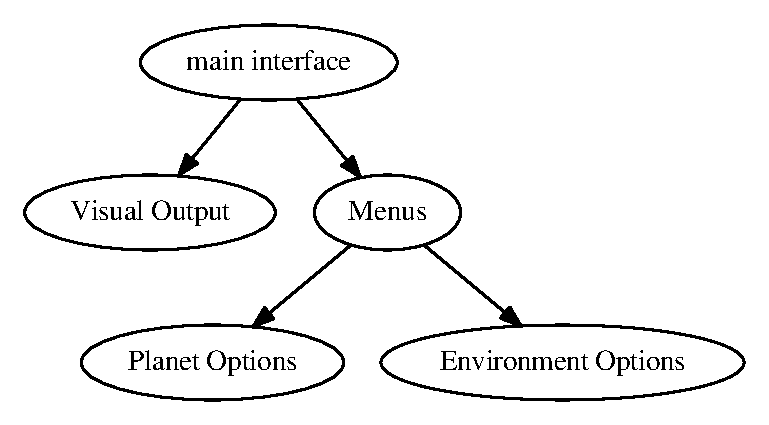
\includegraphics[width=\textwidth]{./img/hier.eps}
\end{figure}

%%%
\section{Class Definitions}
Object oriented programming in Lisp works differently than it does in other
languages, so some things, such as private and public attributes aren't used. 

\subsection{Point} The point class is used to describe anything with X and Y
values, so positions and velocities. It's attributes are:
\begin{description}[\parindent]
	\item[X] - The X value of the point, stored as a number.
	\item[Y] - The Y value of the point, stored as a number.
\end{description}

\subsection{Body} The body class is used to describe any body in space. This
could be the Sun or a planet. It's attributes are:
\begin{description}[\parindent]
	\item[pos] - The current position of the body in space, stored as a
		point with X and Y values.
	\item[vel] - The current velocity of the body, also stored as a point.
	\item[mass] - The mass of the body, stored as a number.
	\item[size] - The size that the body will be displayed as.
	\item[colour] - The colour that the body will be displayed as.
	\item[id] - An Identifier for each instance of the class.
\end{description} \\

%%%
\section{Storage and Distribution}

In its current state, the program takes up 65MB when compiled. I expect that
this will be higher when I have completed the program but I would think that it
would be no more than 100MB\@. The reason that the executable is so large for a
small program is that the Lisp interpreter that I am using compiles itself and
all of the libraries I use into the executable, which means that the program
should run on any computer without having to install any extra software. \\

The program will be stored on the computer that it is running on, and since it
will be running on a school computer, and I cannot install software on the
school computers I will need to ask one of the schools I.T technicians to
install it for me. \\

I would like to distribute my software via the internet, but due to its large
size it will be easier for me to take it into school on a memory stick to be
installed on a school computer. I can still have the file available for
download, for if a student wishes to use the program themselves. I would also
like to have the programs source code available for download, so a more
technically inclined student could experiment further. Also having the source
code available means that people can see exactly what the program does before
they decide to run it, so they can be sure that I am not trying to do anything
malicious with their computer. \\

\subsection{File Organisation}

The system has very few separate files. The executable, which is the only file
distributed, can be placed anywhere that is convenient for the user. The user
can then create new files from within the system, which will be saved in the
same directory that the executable is placed. \\


%%%
\section{Testing Plan}

\begin{tabular}{p{0.3\textwidth}p{0.3\textwidth}p{0.4\textwidth}} 
	Description & Typical, Erroneous, Extreme & Expected Outcome \\ \hline
	Starting the program & Typical & The program will start \\ 
	Closing the program & Typical & The program will close \\
	Running the simulation & Typical & The simulation will run as expected
	\\
	 & Extreme & The simulation will run as expected \\
	Adding a body & Typical & A body will be added to the system \\
	 & Erroneous & An Error message will show \\
	 & Extreme & A body will be added \\
	Removing a body & Typical & A body will be removed \\
	 & Erroneous & An error message will show \\
	Saving the system to a file & Typical & The system will be save \\
	 & Erroneous & An error message will show \\
	 & Extreme & A warning message will show \\
	Loading the system from a file & Typical & The saved system will be
	loaded \\
	 & Erroneous & An error message will show \\
	 & Extreme & The system will be loaded \\
		
\end{tabular}
